\section{Tower design}

\subsection{Summary of the design}

Once the rotor design has been completed, it is possible to assess the structural properties of the wind turbine's tower. The process is divided in two phases: first, the reference tower is linearly scaled in height, section diameter, and wall thickness. Then, by computing the thrust produced by the rotor, the stresses inside the tower are estimated, and it is checked that the safety factor is satisfactory, and that the fist natural frequency of the system is sufficiently high.

\subsection{Supporting material, analyses and rationale}

In order to compute stresses in the blade, thrust must be computed fist. The highest value of thrust is obtained at the rated wind speed (\cite{hau}), thus it is chosen to use such condition to asses the tower design. 
To compute thrust, the BEM code is used again to compute the induction factor $a$. Then, lift and drag distributions are computed, starting from the definition of the angle of attack $\alpha$:

\begin{equation}
    \alpha = \phi - \beta + \theta 
\end{equation}

where:

\begin{equation}
    \phi = \arctan\left(\frac{V(1 - a)}{ \Omega r}\right)
\end{equation}

The actual velocity at the blade airfoil is computed as:

\begin{equation}
    V = \sqrt{ (V ( 1 - a )) ^ 2 + ( \Omega r ) ^ 2}
\end{equation}

Lift and drag per unit span are computed as:

\begin{equation}
    \frac{dL_a}{dr} = \frac{1}{2} \rho V ^ 2 C_l c;
\end{equation}

\begin{equation}
    \frac{dD_a}{dr}  = \frac{1}{2} \rho V ^ 2 C_d c;
\end{equation}

and finally, forces in the edge and flap directions are computed as:

\begin{equation}
    \frac{dF_y}{dr}  = dL_a \sin(\phi) - dD_a \cos(\phi);
\end{equation}

\begin{equation}
    \frac{dF_z}{dr}  = dL_a \cos(\phi) + dD_a \sin(\phi);
\end{equation}

The total value of thrust per blade is computed by integrating the force in the $z$ direction:

\begin{equation}
    F_z = \int_{0}^{R} \frac{dF_z}{dr} dr
\end{equation}

The final value of thrust is computed at rated conditions:

\begin{align}
    T &= 3 F_z \\
    &= 308 kN \\ \nonumber
\end{align}

At this point, stresses are computed in the tower by applying simple beam theory. The sectional properties of the tower and the stresses in the tower's wall are computed as presented in \cite{Bispl} as a function of height $h$. Maximum stresses are supposed to be equal to the summation of gravitational and bending stresses, the latter being the most severe. The value of the stress in the tower is computed as:

\begin{equation}
    \sigma = \frac{N}{A} + \frac{M r_{ext}}{I}
\end{equation}

\begin{figure}[H]
\centering
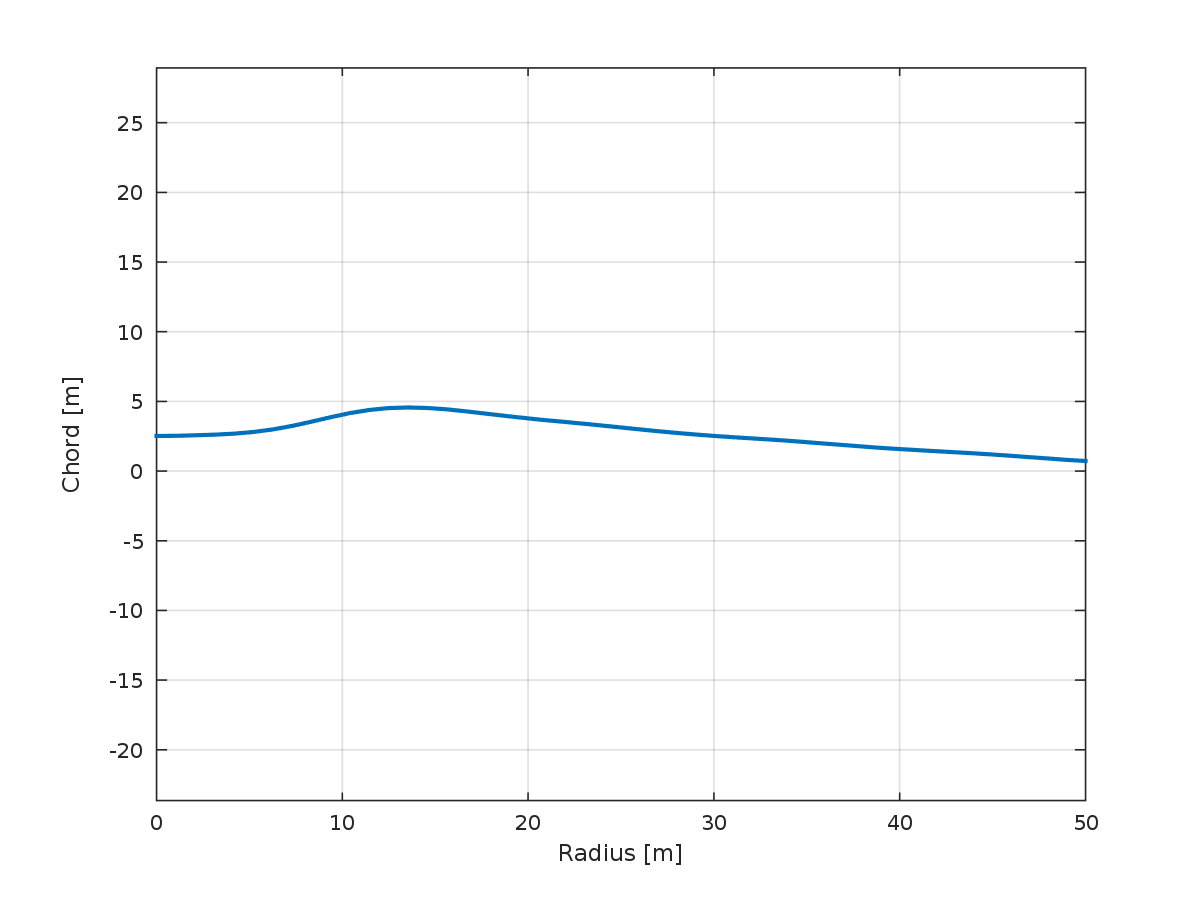
\includegraphics[width=0.7\textwidth]{Images/chord.png} 
\caption{Chord distribution}\label{fig:chord}
\end{figure}